\documentclass{article}
\usepackage[utf8]{inputenc}
\usepackage{graphicx}
\usepackage{dirtytalk}
\usepackage{caratula}
\usepackage{amssymb}
\usepackage{amsmath}
\usepackage{geometry}
\usepackage{fixltx2e}
\usepackage{cite}
\usepackage{float}
\geometry{
 a4paper,
 total={210mm,297mm},
 left=30mm,
 right=30mm,
 top=30mm,
 bottom=30mm,
 }
\begin{document}
% Estos comandos deben ir antes del \maketitle
\materia{Métodos Numéricos} % obligatorio

\titulo{Trabajo Práctico 2} % obligatorio
\subtitulo{Si nos organizamos aprobamos todos...} % opcional
\grupo{El siguiente trabajo consiste en la implementación de algoritmos que reciben una imagen y deciden qué dígito representa. Para ello se implementa el algoritmo de KNN, con una reducción de dimensión previa utilizando PCA.
A la vez con el objetivo de tener la descomposición en valores singulares implementamos el algoritmo de Método de la Potencia con Deflación para la estimación de Autovalores y Autovectores de la Matriz de Covarianza.       
\\
}
\integrante{Bayardo Julián}{850/13}{julian@bayardo.com.ar} % obligatorio
\integrante{Carrasco Manuel}{646/13}{mgcarrasco2012@gmail.com} % obligatorio 
\integrante{Gómez Fabián}{799/13}{fabiandagomez@hotmail.com} % obligatorio 
\integrante{Keegan Maureen}{761/13}{maukeegan@hotmail.com} % obligatorio 
 



\maketitle






 
\pagebreak
%\newpage

\section*{Introducción Teórica}{} 

$\ $ $\ $ $\ $ $\ $Con la intención de corregir exámenes automáticamente, la cátedra nos ha delegado el problema de interpretar dígitos manuscritos. 
Para su resolución, optamos por implementar dos métodos: k-vecinos más cercanos y análisis de componentes principales.
En ambas implementaciones utilizamos una base de entrenamiento de imágenes que contiene, para cada una de ellas, el dígito al que corresponde. De esta manera, para procesar un nuevo dígito, podemos comparar la nueva imagen con las que ya conocemos y decidir a qué dígito pertenece. Más adelante veremos cómo realizar esta comparación.

El algoritmo de los k vecinos más cercanos (kNN por su nombre en inglés) consiste en obtener las distancias entre las imágenes de la base de entrenamiento y la imagen de testeo. Luego se elige las k imágenes que den menor distancia y se determina cuál etiqueta entre ellas es la más popular. Esa etiqueta es la que se devuelve como resultado.

Dado que la complejidad de este algoritmo crece en relación al tamaño de las imágenes y a la cantidad de imágenes de testeo y de entrenamiento, el cómputo se vuelve costoso con rapidez. Para solucionar este inconveniente, utilizamos el método de análisis de componentes principales (PCA por su nombre en inglés). Este algoritmo sintetiza la información relevante de la imagen, eliminando aquellas partes que no la distinguen de las otras. De esta manera se reduce la cantidad de componentes de cada elemento a comparar, disminuyendo la complejidad del cálculo de distancia entre imágenes.


Si bien planteamos cómo podríamos resolver el problema, no es posible saber si la resolución es correcta sin conocer cuál debería ser la solución. Es decir, al procesar una imagen, necesitamos saber qué dígito representa para poder evaluar si nuestro algoritmo efectivamente lo reconoció. De este modo podemos calcular la eficiencia del método. Es por esto que se aplica la técnica de \textit{K-fold cross validation}, que consiste en particionar la base de training dada y utilizar una parte como la nueva base de entrenamiento y el resto como testing.



\pagebreak



\section*{Desarrollo}{}

$\ $ $\ $ $\ $ $\ $La primera decisión que tomamos fue levantar los datos de entrada  divididos en dos estructuras. Por un lado creamos una matriz que tiene como filas a las distintas imágenes, y por el otro, guardamos en un vector las etiquetas asociadas a cada imagen, en el mismo orden relativo que tienen las imágenes en la matriz. De este modo nos aseguramos que las etiquetas no se verán afectadas por las operaciones sobre las imágenes. Como estructura de datos para dicha matriz utilizamos un vector de vectores.

El siguiente paso fue la implementación de kNN. En esta primera instancia consideramos los datos con su tamaño original. Para cada imagen del testing calculamos su distancia con las imágenes del training utilizando una norma que se toma como parámetro. Es decir el usuario puede variar dicho parámetro a gusto. 

Para poder tomar las k distancias mínimas de forma eficiente, optamos por usar un MinHeap que vaya guardando las distancias obtenidas. Luego, calculamos la etiqueta más popular y la devolvemos como resultado.

Dado que la complejidad del algoritmo de kNN crece en función del tamaño de las imágenes y la cantidad de imágenes de training y de testing, se vuelve inviable usar este algoritmo para gran cantidad de datos o imágenes de gran tamaño. Es necesario entonces reducir de alguna manera el tamaño de los datos para el funcionamiento apropiado del algoritmo. Para ello se utiliza el algoritmo de PCA, que se encarga de tomar los $\alpha$ valores que más representan a cada imagen.

Para implementar PCA nuestro primer problema fue encontrar la matriz de covarianza. Para eso consideramos la matriz X $\in$ $\mathbb{R}^{nxm}$  de manera tal que:

\begin{align*}
fila_i(X)=(x^{(i)} - \mu)^t/\sqrt{n -1}
\end{align*}

donde x$^{(i)}$ es la i-ésima imagen de la base de entrenamiento, $\mu$ es el vector promedio de dichas imágenes, y n es la cantidad de imágenes.
Si multiplicamos X$^t$X encontramos la matriz que buscábamos. La matriz M$x$ contiene en la posición $(k,k)$ la varianza muestral de la componente k de todas las imágenes y en la posición $(k, j)$ la covarianza de la componente k y la componente j. Es decir:

\begin{align*} 
Mx_{k,j} =
\left\{
	\begin{array}{ll}
		\frac{1}{n-1}\sum_{i=1}^{n} (x^{(i)}_k - \mu_k)^2 & \mbox{si } k = j\\
		& \\
		\frac{1}{n-1}\sum_{i=1}^{n} (x^{(i)}_k - \mu_k)(x^{(i)}_j - \mu_j) & \mbox{si } k \neq j
	\end{array}
\right.
\end{align*}



El costo de calcular esta matriz es muy alto y nos generó problemas a la hora de testear. Para minimizarlos, optamos por dos estrategias distintas. Por un lado, aprovechamos la simetría de la matriz(ya que M$x$ = X$^t$X ), calculando sólamente la mitad, y luego copiando el resto. Por el otro, para mejorar el rendimiento al correr el mismo test varias veces, chequeamos si la matriz de covarianza fue calculada previamente. Si lo fue, la levantamos de un archivo y operamos normalmente; si no, la calculamos y la guardamos en un archivo para su futura utilización. Esto nos permitió corregir errores y realizar pruebas con un mismo caso en menor tiempo.


Para encontrar los autovectores necesarios para la transformación característica planteada, calculamos $\alpha$ autovectores de M$x$. Veamos por qué esto vale.

Sea X = U$\Sigma$V$^t$ la factorización en valores singulares de X, donde U $\in$ $\mathbb{R}^{nxn}$ y V $\in$ $\mathbb{R}^{mxm}$ son matrices ortogonales, y $\Sigma$ $\in$ $\mathbb{R}^{nxm}$. Sabemos que V$^t$ tiene por filas a los autovectores de X$^t$X, es decir, a los autovectores de M$x$.

Para calcular dichos autovectores aplicamos el algoritmo de método de la potencia con deflación $\alpha$ veces. Decidimos que este algoritmo reciba como parámetro la cantidad de iteraciones que va a hacer antes de devolver un resultado. De esta manera el usuario puede decidir qué parámetro pasar para mejorar la precisión en el cálculo de los autovectores. A la vez dimos la posibilidad de que tras una ejecución se devuelva tanto el autovector, como el autovalor asociado a él, ya que el método los va calculando a la vez. Al igual que en kNN, en el método de la potencia también se pasa por parámetro la norma que se quiere utilizar.

Ya calculados los primeros $\alpha$  autovectores de M$x$ (v$_1^t$, ... , v$_\alpha^t$), los usamos para obtener la transformación lineal:

\begin{align*}
tc(x_i) = (v_1^t*x_i, ... , v_\alpha^t*x_i)
\end{align*}

que extrae las $\alpha$ componentes principales del vector x$_i$ y las cambia de base(recordar que como las filas de V$^t$ forman una base ortonormal de vectores, V$^t$X$^t$, equivale a cambiar de base a X$^t$). 
En el nuevo sistema de coordenadas la varianza de mayor tamaño del conjunto de datos original es capturada en el primer eje, la segunda varianza más grande es el segundo eje, y así sucesivamente hasta el eje $\alpha$. Además, la covarianza entre las variables es 0.

%Esto nos permite aplicarle dicha transformación lineal a la base de entrenamiento y a la de testing, convirtiendo a cada imagen en una de menor dimensión.
Como la transformación característica se le aplica a un vector particular, queremos realizar el proceso para todas las imágenes de training y testing. Para ello realizamos la multiplicación entre la lista de tuplas \textless autovalor,autovector\textgreater  que calculamos y las bases de datos utilizadas. Es decir, obtenemos dos nuevas matrices con la misma cantidad de filas que antes (ya que se corresponde con la cantidad de imágenes), pero que ahora tienen sólamente $\alpha$ columnas (que se corresponde con el tamaño de dichas imágenes).
Es importante notar que mientras no se modifique el training, el proceso se repite sólo para el testing. Es decir, si no cambiamos nuestra base de comparación, sólamente se deben redimensionar las imágenes a testear, de la misma manera que se lo hizo para la base de entrenamiento. De este modo se ahorra tiempo de cómputo si lo que se desea es probar varios testing sets para un mismo training set.

%De este modo obtenemos dos nuevas bases con datos de dimensión menor, más precisamente dimensión de la base de testing es  $\mathbb{R}^{tx \alpha}$ y  la de training queda  $\mathbb{R}^{nx \alpha}$. Este procedimiento solo debe realizarse una vez para el training, si se quieren probar varios testing con un mismo set de training.

Una vez hecho esto, aplicamos el algoritmo de kNN para terminar de resolver el problema general. Podemos ver entonces que, dependiendo del $\alpha$ elegido, el algoritmo será mucho más eficiente que el que utiliza los datos originales.

%Tras terminar toda la implementación para resolver el problema de reconocimiento de caracteres, queremos intentar ver cuán efectivo es nuestro algoritmo. Con esta intención, se busca aplicar la técnica de K-Fold Cross Validation que consta en dividir en dos los datos de entrada que en el algoritmo original se usaban como training test.
Por último, implementamos K-Fold Cross Validation, que consiste en particionar la base de entrenamiento en dos nuevas bases: una de entrenamiento y una de testing. De este modo, conocemos los resultados esperados para cada imagen, y los guardamos en un vector, para poder luego compararlos con los resultados obtenidos. Si se quiere entonces probar la efectividad de un método, se debe aplicar K-Fold Cross Validation, y luego llamar a los métodos con las nuevas bases de training y de testing.

Para levantar los datos de todos los archivos tuvimos un problema con la función .substr porque pensábamos que tomaba una posición de inicio y una de fin, y en realidad tomaba una posición de inicio y una longitud. 



A lo largo de este desarrollo hemos planteado distintas hipótesis que pasaremos a probar o desestimar en la sección de Resultados.
\begin{itemize}
  \item La aplicación de PCA mejora la complejidad temporal del algoritmo kNN, al disminuir las dimensiones de los elementos a comparar. 
  \item Distintos tipos de $\alpha$ tomados para PCA conllevan a distintos tiempos de ejecución y a la vez a distinto hit-rate al analizar la efectividad del algoritmo.
  \item La cantidad de vecinos a comparar del algoritmo de kNN puede llegar a afectar la efectividad a la hora de resolver el problema general.
  \end{itemize}
  
  
  Llegando al final del desarrollo del algoritmo no tuvimos mucho tiempo de realizar experimentos para probar dichas hipótesis planteadas. Aunque las bases teóricas avalen nuestras ideas, sabemos que una mala implementación de los algoritmos planteados puede llegar a traer malos resultados finales que no pudimos corroborar bien.
  
  Nuestra idea de qué puede ser los cálculos de los autovalores o el cálculo de la matriz de covarianza. Viendo esto, igual quisimos probar el hit/miss rate y nos dió un valor de $67\%$
 

\section*{Resultados}{}
\begin{figure}[H]
\centering
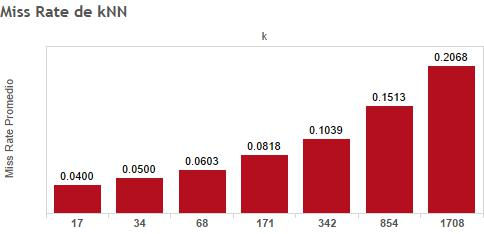
\includegraphics[scale=0.90]{MissRatedekNN.jpg}
\caption{Miss Rate de kNN. Miss Rate en función de k.}
\label{fig:MissRatekNN}
\end{figure}

\begin{figure}[H]
\centering
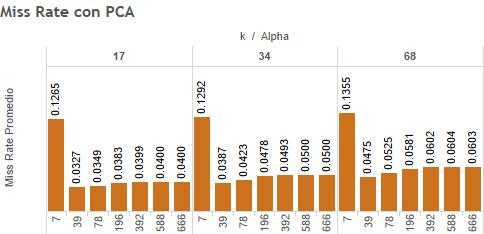
\includegraphics[scale=0.90]{MissRatedePCA.jpg}
\caption{Miss Rate de PCA. (Eje horizontal superior: k. Eje horizontal inferior: alpha)}
\label{fig:MissRatePCA}
\end{figure}


\begin{figure}[H]
\centering
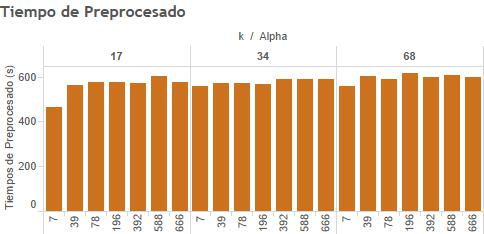
\includegraphics[scale=0.90]{preprocesado.jpg}
\caption{Tiempo de Preprocesado (Eje horizontal superior: k. Eje horizontal inferior: alpha)}
\label{fig:Preprocesado}
\end{figure} 

\pagebreak


\section*{Discusión}{}



\subsection*{Consideraciones para los experimentos.}

Para explicar la elección de los valores de k debemos primero dar una pequeña introducción.  Para ello calculamos la cantidad de apariciones de cada dígito en el training set y este fue el resultado:

\begin{figure}[h]
\centering
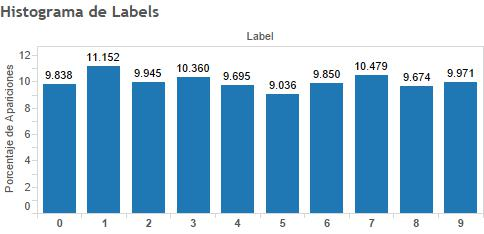
\includegraphics[scale=0.80]{histo.jpg}
\caption{Histograma de labels}
\end{figure}

Entonces el dígito 5 tiene el mínimo porcentaje de apariciones siendo aproximadamente $9.03\%$.  Dividimos el training set en 10 particiones aleatorias y disjuntas utilizando MATLAB. Como la división es aleatoria, asumimos que $9.03$ sigue siendo el porcentaje menor de apariciones. 

Por cada corrida del método, se utiliza una partición de 4200 imágenes como testing set, y las restantes 9 particiones como training set (ejecutando todas las combinaciones).  Entonces para un caso, el nuevo training set contiene 37800 imágenes. El $9.03\%$ de 37800 es un estimativo de la mínima cantidad de apariciones del dígito 5. Es sobre este número que elegimos el k, tomando 7 distintos porcentajes. Trabajar con el mínimo valor de apariciones de un dígito del training set, suponemos que evita caer en problemas de sobreclasificación.


Definimos $min$ = $9.03\%$ de 37800. Los k elegidos para la experimentación son: \newline
\begin{center}
\begin{tabular}{ l | c }
 k & Porcentaje de $min$  \\
1708 & 50\% \\
854 & 25\% \\
342 & 10\% \\
171 & 5\% \\
68 & 2\% \\
34 & 1\% \\
17& 0.5\% \\

\end{tabular}
\end{center}
\\

\subsection*{Resultados kNN-Normal}

La Figura \ref{fig:MissRatekNN} muestra en función de k  los Miss Rate promedio de 10 corridas del método. Para cada una de las 10 corridas, una partición es utilizada como testing set y el resto como training set.

Del gráfico se entiende que el Miss Rate promedio disminuye a medida que el k desciende. Es decir como se obtienen mejores predicciones, al disminuir el k. Los datos obtenidos contradijeron nuestra primera suposición.

Por esa razón, consideramos posible que para la elección de un k óptimo (en este método) no solo se debe tener en cuenta las frecuencias de los dígitos sino también la distancia entre los de un mismo grupo. kNN tiene la particularidad de considerar todos los pixeles de una imagen. En otras palabras, tiene en cuenta también las diferencias entre imágenes de un mismo dígito. Posiblemente considerar solo las frecuencias sea suficiente para el reconocimiento de dígitos escritos por una sola persona. Porque implicaría menor distancia entre imágenes de un mismo dígito.

% FALTA HABLAR DE LOS TIEMPOS
\subsection*{Resultados PCA}

En la experimentación de PCA, variamos tanto el k como el alpha. Los k elegidos son los tres mejores para kNN. Para alpha tomamos 7 porcentajes del tamaño de la imagen. Nuestra hipótesis consiste que para alphas muy grandes, el tiempo de cómputo es considerable y que el miss rate es bajo. En cambio, para alphas más chicos un tiempo de computo bajo acompañado de una peor tasa de predicción. 

En los gráficos correspondientes a la experimentación con PCA, tuvimos la misma metodología que para kNN-Normal. Usando 10 particiones fuimos considerando cada una como testing set y el resto como training set.

La Figura \ref{fig:MissRatePCA} nos provee los resultados de las corridas del método en cuestión. Para cada k hay una sección propia, determinada por el eje horizontal superior. Dentro de cada una, se observan los distintos Miss Rate promedio (eje vertical) por cada alpha posible (eje horizontal inferior). 

El Miss Rate Promedio se comportó igual para todos los k. Disminuir el alpha implicó mejores predicciones hasta cierto punto. Desde el valor 7 para alpha, la calidad de las predicciones empeora. 

Estos resultados confirmaron parte de nuestra hipótesis: no es necesario trabajar con todas las componentes de las imágenes. Es posible obtener mejores predicciones si uno no trabaja con el total de la imágen. 

Nos hace suponer que el análisis de componentes principales de los vectores nos ayuda a descartar los pixeles que no son cruciales para la diferenciación de dígitos y además concentrarnos en las similitudes entre las imágenes de un mismo dígito. Mejorando el escenario desfavorable de kNN-Normal con imágenes muy distintas para un mismo dígito.

% FALTA HABLAR DE LOS TIEMPOS DE COMPUTO


\end{document}